\documentclass{article}\usepackage[]{graphicx}\usepackage[]{color}
% maxwidth is the original width if it is less than linewidth
% otherwise use linewidth (to make sure the graphics do not exceed the margin)
\makeatletter
\def\maxwidth{ %
  \ifdim\Gin@nat@width>\linewidth
    \linewidth
  \else
    \Gin@nat@width
  \fi
}
\makeatother

\definecolor{fgcolor}{rgb}{0.345, 0.345, 0.345}
\newcommand{\hlnum}[1]{\textcolor[rgb]{0.686,0.059,0.569}{#1}}%
\newcommand{\hlstr}[1]{\textcolor[rgb]{0.192,0.494,0.8}{#1}}%
\newcommand{\hlcom}[1]{\textcolor[rgb]{0.678,0.584,0.686}{\textit{#1}}}%
\newcommand{\hlopt}[1]{\textcolor[rgb]{0,0,0}{#1}}%
\newcommand{\hlstd}[1]{\textcolor[rgb]{0.345,0.345,0.345}{#1}}%
\newcommand{\hlkwa}[1]{\textcolor[rgb]{0.161,0.373,0.58}{\textbf{#1}}}%
\newcommand{\hlkwb}[1]{\textcolor[rgb]{0.69,0.353,0.396}{#1}}%
\newcommand{\hlkwc}[1]{\textcolor[rgb]{0.333,0.667,0.333}{#1}}%
\newcommand{\hlkwd}[1]{\textcolor[rgb]{0.737,0.353,0.396}{\textbf{#1}}}%
\let\hlipl\hlkwb

\usepackage{framed}
\makeatletter
\newenvironment{kframe}{%
 \def\at@end@of@kframe{}%
 \ifinner\ifhmode%
  \def\at@end@of@kframe{\end{minipage}}%
  \begin{minipage}{\columnwidth}%
 \fi\fi%
 \def\FrameCommand##1{\hskip\@totalleftmargin \hskip-\fboxsep
 \colorbox{shadecolor}{##1}\hskip-\fboxsep
     % There is no \\@totalrightmargin, so:
     \hskip-\linewidth \hskip-\@totalleftmargin \hskip\columnwidth}%
 \MakeFramed {\advance\hsize-\width
   \@totalleftmargin\z@ \linewidth\hsize
   \@setminipage}}%
 {\par\unskip\endMakeFramed%
 \at@end@of@kframe}
\makeatother

\definecolor{shadecolor}{rgb}{.97, .97, .97}
\definecolor{messagecolor}{rgb}{0, 0, 0}
\definecolor{warningcolor}{rgb}{1, 0, 1}
\definecolor{errorcolor}{rgb}{1, 0, 0}
\newenvironment{knitrout}{}{} % an empty environment to be redefined in TeX

\usepackage{alltt}

\usepackage[OT4]{polski}
\usepackage[utf8]{inputenc}
\usepackage[T1]{fontenc}
\usepackage[top=2.5cm, bottom=2.5cm, left=2cm, right=2cm]{geometry}
\usepackage{graphicx}
\usepackage{float}
\usepackage[colorlinks=true, linkcolor=blue]{hyperref}
\usepackage{amsmath}
\usepackage{amssymb}



\title{Lista 1}
\author{Mikołaj Langner, Marcin Kostrzewa}
\date{31.3.2021}
\IfFileExists{upquote.sty}{\usepackage{upquote}}{}
\begin{document}

\maketitle

\section{Wstęp}
W niniejszym sprawozdaniu zajmować się będziemy danymi dotyczącymi klientów pewnej sieci telefonii komórkowej.
Naszym zadaniem będzie odkrycie zależności między zmiennymi, które określą przyczyny rezygnacji klientów z oferty (churn analysis).

\section{Wczytanie i identyfikacja danych}
Wczytajmy dane z pliku i przeprowadźmy ich wstępną analizę i obróbkę:

\begin{knitrout}
\definecolor{shadecolor}{rgb}{0.969, 0.969, 0.969}\color{fgcolor}\begin{kframe}
\begin{alltt}
\hlstd{df} \hlkwb{<-} \hlkwd{read.csv}\hlstd{(}\hlstr{'churn.txt'}\hlstd{,} \hlkwc{stringsAsFactors} \hlstd{=} \hlnum{TRUE}\hlstd{)}
\hlstd{df}\hlopt{$}\hlstd{Area.Code} \hlkwb{=} \hlkwd{as.factor}\hlstd{(df}\hlopt{$}\hlstd{Area.Code)}
\end{alltt}
\end{kframe}
\end{knitrout}

\begin{itemize}

\item poznajmy rozmiar naszych danych:
\begin{knitrout}
\definecolor{shadecolor}{rgb}{0.969, 0.969, 0.969}\color{fgcolor}\begin{kframe}
\begin{alltt}
\hlkwd{dim}\hlstd{(df)}
\end{alltt}
\begin{verbatim}
## [1] 3333   21
\end{verbatim}
\end{kframe}
\end{knitrout}
--- jest 21 zmiennych i 3333 obserwacji;

\item sprawdźmy ich typ:
\begin{table}[!h]

\caption{\label{tab:tabela_1}Typy zmiennych}
\centering
\resizebox{\linewidth}{!}{
\begin{tabular}[t]{l|l|l|l|l|l|l|l|l|l|l|l|l|l|l|l|l|l|l|l|l|l}
\hline
  & State & Account.Length & Area.Code & Phone & Int.l.Plan & VMail.Plan & VMail.Message & Day.Mins & Day.Calls & Day.Charge & Eve.Mins & Eve.Calls & Eve.Charge & Night.Mins & Night.Calls & Night.Charge & Intl.Mins & Intl.Calls & Intl.Charge & CustServ.Calls & Churn.\\
\hline
Typ zmiennej & factor & integer & factor & factor & factor & factor & integer & numeric & integer & numeric & numeric & integer & numeric & numeric & integer & numeric & numeric & integer & numeric & integer & factor\\
\hline
\end{tabular}}
\end{table}


Zmienna `Churn.` mówi o tym, czy dany klient zrezygnował z oferty.

\item sprawdźmy czy pojawiają się wartości brakujące:
\begin{knitrout}
\definecolor{shadecolor}{rgb}{0.969, 0.969, 0.969}\color{fgcolor}\begin{kframe}
\begin{alltt}
\hlkwd{sum}\hlstd{(}\hlkwd{sapply}\hlstd{(df,} \hlkwa{function}\hlstd{(}\hlkwc{x}\hlstd{)} \hlkwd{sum}\hlstd{(}\hlkwd{is.na}\hlstd{(x))))}
\end{alltt}
\begin{verbatim}
## [1] 0
\end{verbatim}
\end{kframe}
\end{knitrout}
--- nie ma więc brakujących obserwacji;
\item usuńmy dane pełniące rolę indentyfikatora (numer telefonu):
\begin{knitrout}
\definecolor{shadecolor}{rgb}{0.969, 0.969, 0.969}\color{fgcolor}\begin{kframe}
\begin{alltt}
\hlstd{df} \hlkwb{<-} \hlkwd{subset}\hlstd{(df,} \hlkwc{select}\hlstd{=}\hlopt{-}\hlstd{Phone)}
\end{alltt}
\end{kframe}
\end{knitrout}

\end{itemize}

\section{Analiza zmiennych, szkanie zależności}
Teraz podzielimy zmienne ze względu na ich typ oraz wykonamy kilka wykresów, które pomogą w zauważeniu pewnych zależności i wyborze najistotniejszych pod względem naszej analizy atrybutów.
\begin{knitrout}
\definecolor{shadecolor}{rgb}{0.969, 0.969, 0.969}\color{fgcolor}\begin{kframe}
\begin{alltt}
\hlcom{# wczytanie potrzebnych bibliotek}
\hlkwd{library}\hlstd{(ggplot2)}
\hlkwd{library}\hlstd{(ggmosaic)}
\hlkwd{library}\hlstd{(GGally)}
\hlkwd{library}\hlstd{(tidyr)}
\hlkwd{library}\hlstd{(dplyr)}
\hlkwd{library}\hlstd{(EnvStats)}
\hlkwd{library}\hlstd{(DescTools)}
\hlkwd{library}\hlstd{(moments)}
\end{alltt}
\end{kframe}
\end{knitrout}


\begin{knitrout}
\definecolor{shadecolor}{rgb}{0.969, 0.969, 0.969}\color{fgcolor}\begin{kframe}
\begin{alltt}
\hlstd{factors} \hlkwb{<-} \hlkwd{subset}\hlstd{(df,} \hlkwc{select}\hlstd{=}\hlkwd{sapply}\hlstd{(df, is.factor))}
\hlstd{numerics} \hlkwb{<-} \hlkwd{subset}\hlstd{(df,} \hlkwc{select}\hlstd{=}\hlkwd{sapply}\hlstd{(df,} \hlkwa{function}\hlstd{(}\hlkwc{x}\hlstd{)} \hlopt{!}\hlkwd{is.factor}\hlstd{(x)))}
\end{alltt}
\end{kframe}
\end{knitrout}

Sprawdźmy zależności pomiędzy zmiennymi ciągłymi.
\begin{knitrout}
\definecolor{shadecolor}{rgb}{0.969, 0.969, 0.969}\color{fgcolor}\begin{kframe}
\begin{alltt}
\hlstd{continuous} \hlkwb{<-} \hlkwd{subset}\hlstd{(numerics,} \hlkwc{select}\hlstd{=}\hlkwd{sapply}\hlstd{(numerics,} \hlkwa{function}\hlstd{(}\hlkwc{x}\hlstd{)} \hlopt{!}\hlkwd{is.integer}\hlstd{(x)))}
\hlkwd{ggpairs}\hlstd{(continuous,}
        \hlkwc{lower}\hlstd{=}\hlkwd{list}\hlstd{(}\hlkwc{continuous}\hlstd{=}\hlkwd{wrap}\hlstd{(}\hlstr{"points"}\hlstd{,} \hlkwc{alpha}\hlstd{=}\hlnum{.4}\hlstd{,} \hlkwc{size}\hlstd{=}\hlnum{.01}\hlstd{)))}
\end{alltt}
\end{kframe}

{\centering 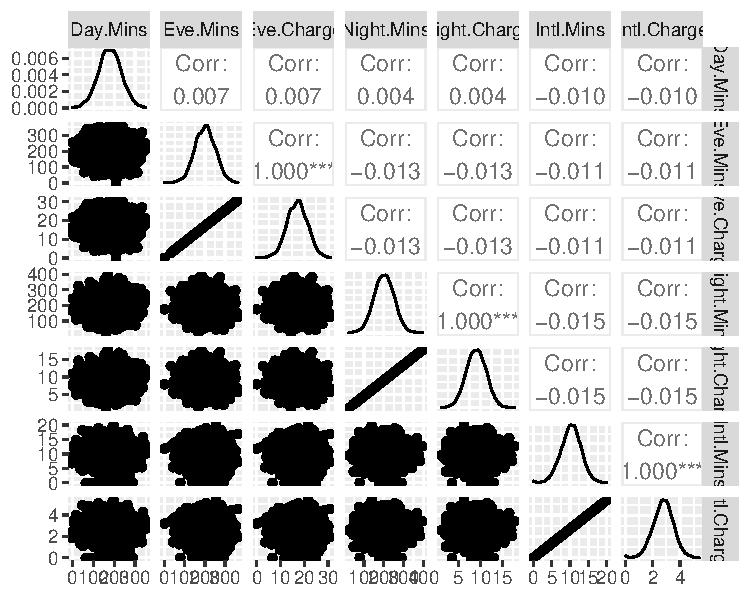
\includegraphics[width=\maxwidth]{figure/Pair_plot_for_continuous_variables-1} 

}



\end{knitrout}
Możemy zauważyć, że zmienne z przyrostkami `.Mins` oraz `.Charge` są ze sobą idealnie skorelowane. Odrzućmy zatem od razu dane z przyrostkiem `.Charge` dla ułatwienia dalszej analizy.

\begin{knitrout}
\definecolor{shadecolor}{rgb}{0.969, 0.969, 0.969}\color{fgcolor}\begin{kframe}
\begin{alltt}
\hlstd{numerics} \hlkwb{<-} \hlkwd{subset}\hlstd{(numerics,} \hlkwc{select}\hlstd{=}\hlopt{-}\hlkwd{c}\hlstd{(Day.Charge, Eve.Charge, Night.Charge, Intl.Charge))}
\end{alltt}
\end{kframe}
\end{knitrout}

\begin{knitrout}
\definecolor{shadecolor}{rgb}{0.969, 0.969, 0.969}\color{fgcolor}\begin{kframe}
\begin{alltt}
\hlstd{numerics} \hlkwb{<-} \hlkwd{data.frame}\hlstd{(numerics,} \hlkwc{Churn.} \hlstd{= df}\hlopt{$}\hlstd{Churn.)}
\end{alltt}
\end{kframe}
\end{knitrout}

\begin{knitrout}
\definecolor{shadecolor}{rgb}{0.969, 0.969, 0.969}\color{fgcolor}\begin{kframe}
\begin{alltt}
\hlkwd{ggplot}\hlstd{(}\hlkwd{gather}\hlstd{(factors,} \hlstr{"key"}\hlstd{,} \hlstr{"value"}\hlstd{,} \hlopt{-}\hlstd{Churn.),} \hlkwd{aes}\hlstd{(value,} \hlkwc{fill}\hlstd{=Churn.))} \hlopt{+}
  \hlkwd{geom_bar}\hlstd{(}\hlkwc{position}\hlstd{=}\hlstr{"fill"}\hlstd{)} \hlopt{+}
  \hlkwd{facet_wrap}\hlstd{(}\hlopt{~}\hlstd{key,} \hlkwc{scales}\hlstd{=}\hlstr{'free'}\hlstd{)}
\end{alltt}
\end{kframe}

{\centering 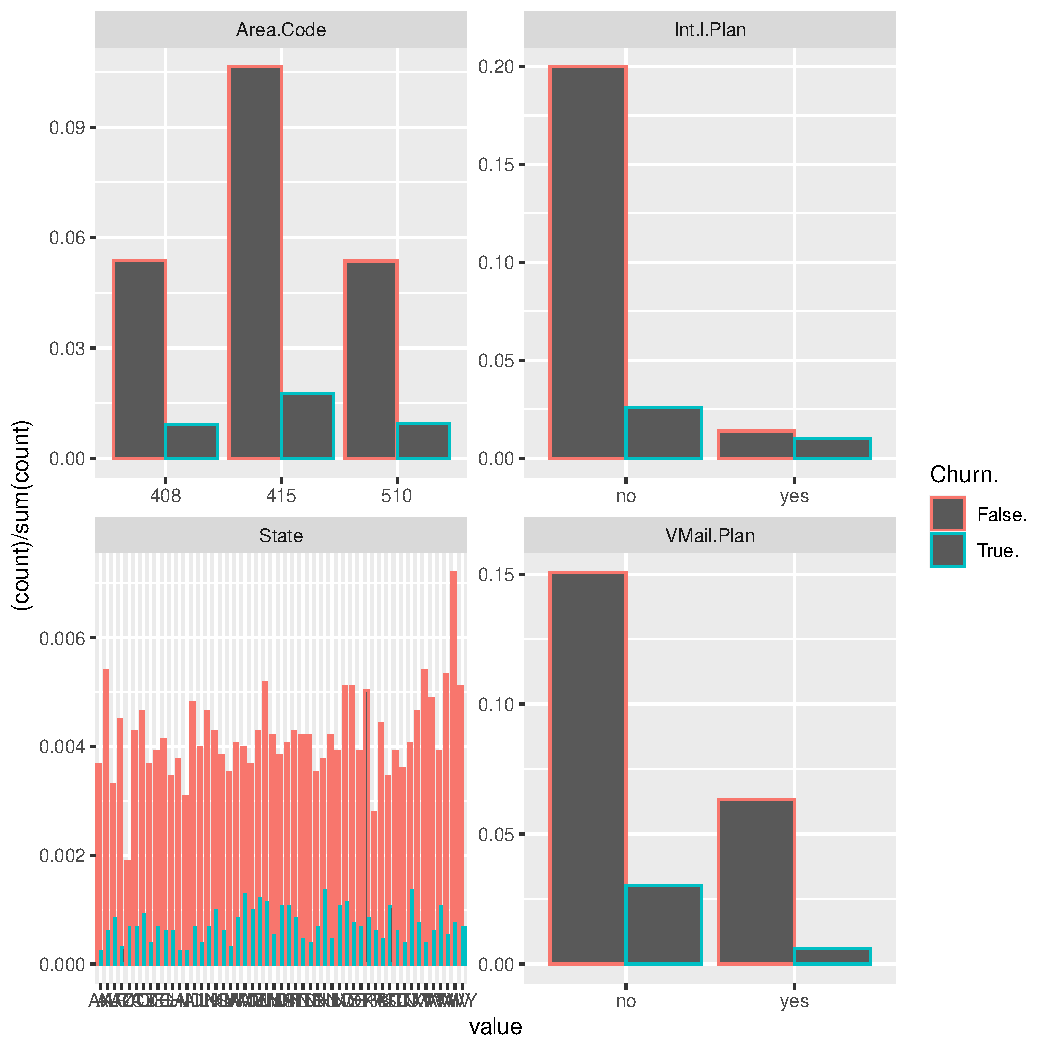
\includegraphics[width=\maxwidth]{figure/Overviews_plots_grouped-1} 

}


\begin{kframe}\begin{alltt}
\hlkwd{ggplot}\hlstd{(}\hlkwd{gather}\hlstd{(numerics,} \hlstr{"key"}\hlstd{,} \hlstr{"value"}\hlstd{,} \hlopt{-}\hlstd{Churn.),} \hlkwd{aes}\hlstd{(}\hlkwc{x}\hlstd{=value,} \hlkwc{color}\hlstd{=Churn.))} \hlopt{+}
  \hlkwd{geom_freqpoly}\hlstd{(}\hlkwd{aes}\hlstd{(}\hlkwc{y}\hlstd{=..density..),} \hlkwc{position}\hlstd{=}\hlstr{"identity"}\hlstd{)} \hlopt{+}
  \hlkwd{facet_wrap}\hlstd{(}\hlopt{~}\hlstd{key,} \hlkwc{scales}\hlstd{=}\hlstr{'free'}\hlstd{)}
\end{alltt}
\end{kframe}

{\centering 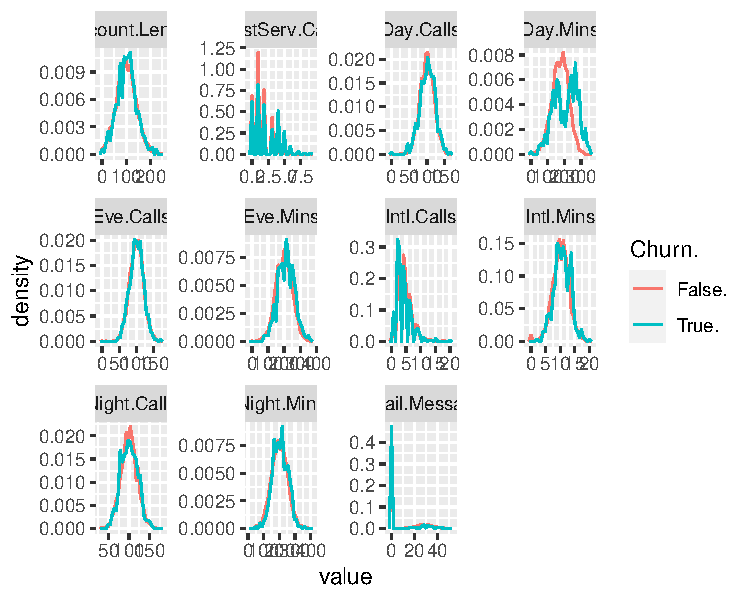
\includegraphics[width=\maxwidth]{figure/Overviews_plots_grouped-2} 

}


\begin{kframe}\begin{alltt}
\hlkwd{ggplot}\hlstd{(}\hlkwd{gather}\hlstd{(numerics,} \hlstr{"key"}\hlstd{,} \hlstr{"value"}\hlstd{,} \hlopt{-}\hlstd{Churn.),} \hlkwd{aes}\hlstd{(value,} \hlkwc{color}\hlstd{=Churn.))} \hlopt{+}
  \hlkwd{geom_boxplot}\hlstd{(}\hlkwd{aes}\hlstd{(}\hlkwc{x}\hlstd{=value))} \hlopt{+}
  \hlkwd{facet_wrap}\hlstd{(}\hlopt{~}\hlstd{key,} \hlkwc{scales}\hlstd{=}\hlstr{'free'}\hlstd{)}
\end{alltt}
\end{kframe}

{\centering 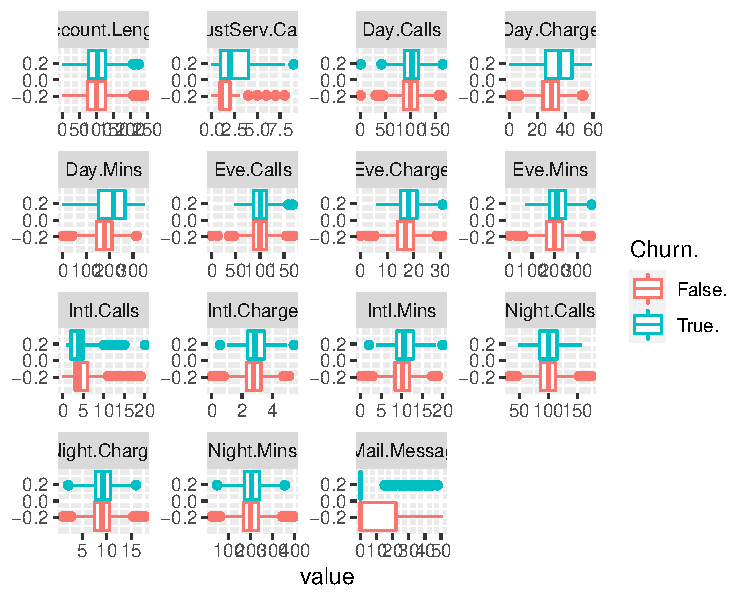
\includegraphics[width=\maxwidth]{figure/Overviews_plots_grouped-3} 

}


\begin{kframe}\begin{alltt}
\hlkwd{ggplot}\hlstd{(}\hlkwd{gather}\hlstd{(numerics,} \hlstr{"key"}\hlstd{,} \hlstr{"value"}\hlstd{,} \hlopt{-}\hlstd{Churn.),} \hlkwd{aes}\hlstd{(value,} \hlkwc{color}\hlstd{=Churn.))} \hlopt{+}
  \hlkwd{stat_ecdf}\hlstd{()} \hlopt{+}
  \hlkwd{facet_wrap}\hlstd{(}\hlopt{~}\hlstd{key,} \hlkwc{scales}\hlstd{=}\hlstr{'free'}\hlstd{)}
\end{alltt}
\end{kframe}

{\centering 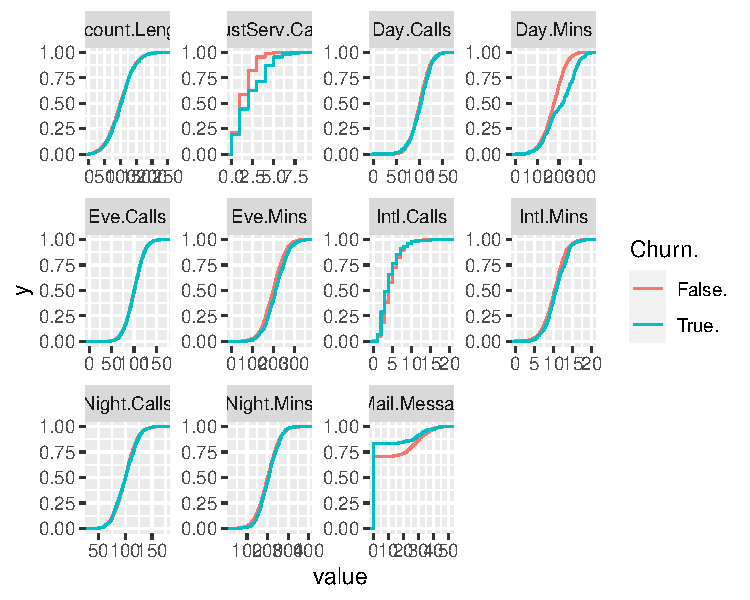
\includegraphics[width=\maxwidth]{figure/Overviews_plots_grouped-4} 

}



\end{knitrout}

By wykryć, dla których zmiennych następuja najważniejsza różnica pomiędzy klientami lojalnymi, a tymi którzy zrezygnowali z usług, posłużymy się również testem Kołmogorova-Smirnova. Poniżej znajduje się funkcja, która wyznacza wyniki tego testu dla naszych zmiennych. 
\begin{knitrout}
\definecolor{shadecolor}{rgb}{0.969, 0.969, 0.969}\color{fgcolor}\begin{kframe}
\begin{alltt}
\hlstd{churn.kstest} \hlkwb{<-} \hlkwa{function}\hlstd{(}\hlkwc{feature}\hlstd{) \{}
  \hlstd{yes} \hlkwb{<-} \hlkwd{subset}\hlstd{(numerics,} \hlkwc{subset}\hlstd{=Churn.}\hlopt{==}\hlstr{"True."}\hlstd{)}
  \hlstd{no} \hlkwb{<-} \hlkwd{subset}\hlstd{(numerics,} \hlkwc{subset}\hlstd{=Churn.}\hlopt{==}\hlstr{"False."}\hlstd{)}
  \hlkwd{return}\hlstd{(}\hlkwd{c}\hlstd{(}\hlkwd{ks.test}\hlstd{(yes[[feature]], no[[feature]])[}\hlkwd{c}\hlstd{(}\hlstr{"statistic"}\hlstd{,} \hlstr{"p.value"}\hlstd{)]))}
\hlstd{\}}
\end{alltt}
\end{kframe}
\end{knitrout}

Tabela poniżej zbiera wyniki przeprowadzonych testów statystycznych.
\begin{table}[!h]

\caption{\label{tab:tabela_3}Wyniki testu Kolmogorova-Smirnova}
\centering
\resizebox{\linewidth}{!}{
\begin{tabular}[t]{l|r|r|r|r|r|r|r|r|r|r|r}
\hline
Zmienna & Account.Length & VMail.Message & Day.Mins & Day.Calls & Eve.Mins & Eve.Calls & Night.Mins & Night.Calls & Intl.Mins & Intl.Calls & CustServ.Calls\\
\hline
statistic & 0.0389430 & 0.1298071 & 0.3172082 & 0.0556326 & 0.1166198 & 0.0192285 & 0.0551378 & 0.0401351 & 0.1007606 & 0.1054201 & 0.2404511\\
\hline
pvalue & 0.5581609 & 0.0000018 & 0.0000000 & 0.1550801 & 0.0000264 & 0.9980118 & 0.1622501 & 0.5189055 & 0.0004560 & 0.0002062 & 0.0000000\\
\hline
\end{tabular}}
\end{table}


Możemy zauważyć, że testy na największe różnice(duża wartość zmiennej \verb|statistic|) wskazują w przypadku zmiennych: CustServ.Calls, Day.Mins, Eve.Mins, 

Po przeanalizowaniu wykresów, decydujemy się na dalszą analizę następujących zmiennych: 
\begin{itemize}
  \item ilościowych:
    \begin{itemize}
    \item CustServ.Calls,
    \item Day.Mins,
    \item Eve.Mins;
    \end{itemize}
  \item jakościowych
    \begin{itemize}
    \item Int.l.Plan,
    \item VMail.Plan,
    \item Churn.
    \end{itemize}
\end{itemize}

\section{Analiza wybranych zmiennych}
Skupmy się jedynie na wybranych zmiennych:
\begin{knitrout}
\definecolor{shadecolor}{rgb}{0.969, 0.969, 0.969}\color{fgcolor}\begin{kframe}
\begin{alltt}
\hlstd{important} \hlkwb{<-} \hlkwd{subset}\hlstd{(df,} \hlkwc{select}\hlstd{=}\hlkwd{c}\hlstd{(CustServ.Calls, Day.Mins, Eve.Mins, Int.l.Plan,}
                                 \hlstd{VMail.Plan, Churn.))}
\end{alltt}
\end{kframe}
\end{knitrout}

Wyznaczmy dla nich wskaźniki sumaryczne.

\begin{knitrout}
\definecolor{shadecolor}{rgb}{0.969, 0.969, 0.969}\color{fgcolor}\begin{kframe}
\begin{alltt}
\hlstd{my_summary} \hlkwb{<-} \hlkwa{function}\hlstd{(}\hlkwc{x}\hlstd{) \{}
  \hlstd{statistics} \hlkwb{<-} \hlkwd{c}\hlstd{(}\hlkwd{mean}\hlstd{(x),} \hlkwd{quantile}\hlstd{(x,} \hlnum{0.25}\hlstd{),} \hlkwd{median}\hlstd{(x),} \hlkwd{quantile}\hlstd{(x,} \hlnum{0.75}\hlstd{),}
                  \hlkwd{IQR}\hlstd{(x),} \hlkwd{min}\hlstd{(x),} \hlkwd{max}\hlstd{(x),} \hlkwd{var}\hlstd{(x),} \hlkwd{sd}\hlstd{(x),} \hlkwd{kurtosis}\hlstd{(x),} \hlkwd{skewness}\hlstd{(x))}
  \hlkwd{names}\hlstd{(statistics)} \hlkwb{<-} \hlkwd{c}\hlstd{(}\hlstr{"Srednia"}\hlstd{,} \hlstr{"Q1"}\hlstd{,} \hlstr{"Mediana"}\hlstd{,} \hlstr{"Q3"}\hlstd{,} \hlstr{"IQR"}\hlstd{,} \hlstr{"Min"}\hlstd{,} \hlstr{"Max"}\hlstd{,}
                         \hlstr{"Wariancja"}\hlstd{,} \hlstr{"Odchylenie standardowe"}\hlstd{,} \hlstr{"Kurtoza"}\hlstd{,} \hlstr{"Skosnosc"}\hlstd{)}
  \hlkwd{return}\hlstd{(statistics)}
\hlstd{\}}
\end{alltt}
\end{kframe}
\end{knitrout}

\begin{table}[!h]

\caption{\label{tab:tabela_2}Wskazniki sumaryczne dla wybranych zmiennych}
\centering
\resizebox{\linewidth}{!}{
\begin{tabular}[t]{l|r|r|r|r|r|r|r|r|r|r|r}
\hline
  & Srednia & Q1 & Mediana & Q3 & IQR & Min & Max & Wariancja & Odchylenie standardowe & Kurtoza & Skosnosc\\
\hline
CustServ.Calls & 1.562856 & 1.0 & 1.0 & 2.0 & 1.0 & 0 & 9.0 & 1.730517 & 1.315491 & 4.726519 & 1.0908683\\
\hline
Day.Mins & 179.775097 & 143.7 & 179.4 & 216.4 & 72.7 & 0 & 350.8 & 2966.696486 & 54.467389 & 2.978290 & -0.0290640\\
\hline
Eve.Mins & 200.980348 & 166.6 & 201.4 & 235.3 & 68.7 & 0 & 363.7 & 2571.894016 & 50.713844 & 3.023792 & -0.0238667\\
\hline
\end{tabular}}
\end{table}



\section{Podsumowanie}


\end{document}
